\documentclass[tikz, border=10pt]{standalone}
\usepackage{tikz}
\usepackage{amsmath}
\usepackage{amssymb}
\usetikzlibrary{calc, arrows.meta}

% Schematic reliability diagram: P(Y = 1 | p_hat = q) against q for a
% perfectly calibrated estimator (the diagonal) and an overconfident one,
% whose values are pushed toward 0 and 1. Thresholding the overconfident
% estimate at p* = 0.09 cuts at a true frequency of about 0.22.
\begin{document}
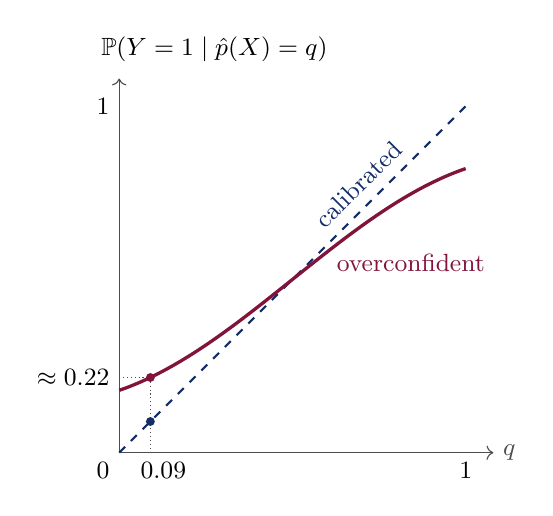
\begin{tikzpicture}[font=\sffamily, x=4.4cm, y=4.4cm,
    lbl/.style={font=\small}]
  \definecolor{calib}{HTML}{142D69}
  \definecolor{overc}{HTML}{82143C}

  \draw[->, black!70] (0, 0) -- (1.08, 0) node[right, lbl] {$q$};
  \draw[->, black!70] (0, 0) -- (0, 1.08);
  \node[lbl, anchor=south west] at (-0.08, 1.1)
    {$\mathbb{P}(Y = 1 \mid \hat{p}(X) = q)$};
  \node[below left, lbl] at (0, 0) {$0$};
  \node[below, lbl] at (1, 0) {$1$};
  \node[left, lbl] at (0, 1) {$1$};

  % Perfect calibration.
  \draw[dashed, thick, calib] (0, 0) -- (1, 1);
  \node[lbl, calib, anchor=south east, rotate=45] at (0.86, 0.87) {calibrated};

  % Overconfident estimator.
  \draw[very thick, overc] (0, 0.18) .. controls (0.35, 0.30) and (0.65, 0.70)
    .. (1, 0.82);
  \node[lbl, overc, anchor=north west] at (0.6, 0.6) {overconfident};

  % The threshold 0.09 of the opening example, read on both curves. The
  % figure comes before p* is defined, so it shows the number.
  \draw[densely dotted, black!70] (0.09, 0) -- (0.09, 0.217);
  \draw[densely dotted, black!70] (0, 0.217) -- (0.09, 0.217);
  \fill[overc] (0.09, 0.217) circle (1.6pt);
  \fill[calib] (0.09, 0.09) circle (1.6pt);
  \node[below, lbl, anchor=north west, inner xsep=0pt] at (0.06, 0) {$0.09$};
  \node[left, lbl] at (0, 0.217) {$\approx 0.22$};
\end{tikzpicture}
\end{document}
